\section{Final held-out evaluation}
After the T06 freeze and reported TA authorization, T07 evaluated the three frozen bundles once on the 340-record Stage~1 test partition. The evaluator used saved features, outcomes, and IDs in their existing row order; no tuning or refitting used test labels. Ranking, calibration, and threshold metrics are reported separately. Table~\ref{tab:test-rank} includes seeded percentile paired-row-bootstrap 95\% intervals (1,000 replicates, seed 42); Table~\ref{tab:test-cal} presents probabilities; Table~\ref{tab:test-threshold} gives confusion matrices at the frozen development thresholds.

\begin{table}[H]\centering\small
\caption{Held-out ranking results and bootstrap 95\% confidence intervals.}\label{tab:test-rank}
\begin{tabular}{lrrr}\toprule
Target & AUROC (95\% CI) & AP (95\% CI) & $n$\\\midrule
Death & .8836 [.8321,.9295] & .7108 [.5927,.8086] & 340\\
ZSN & .7266 [.6605,.7859] & .5957 [.4996,.6814] & 340\\
FIBR\_PREDS & .6567 [.5518,.7624] & .1919 [.1180,.3218] & 340\\\bottomrule
\end{tabular}\end{table}

\begin{table}[H]\centering\small
\caption{Held-out probability and calibration metrics for frozen Platt probabilities. Brier baseline uses observed test prevalence.}\label{tab:test-cal}
\begin{tabular}{lrrrrrr}\toprule
Target & Brier & Baseline & BSS & Log loss & ECE & Intercept / slope\\\midrule
Death & .0799 & .1336 & .4021 & .2680 & .0256 & $-.0365/1.0103$\\
ZSN & .1538 & .1918 & .1983 & .4811 & .0438 & $.7212/1.4001$\\
FIBR\_PREDS & .0900 & .0923 & .0258 & .3222 & .0273 & $-.8126/.6032$\\\bottomrule
\end{tabular}\end{table}

\begin{table}[H]\centering\scriptsize
\caption{Held-out classification at frozen T06 thresholds; confusion counts are TN/FP/FN/TP.}\label{tab:test-threshold}
\begin{tabular}{lrrrrrrr}\toprule
Target & Threshold & Sens. & Spec. & Precision & F1 & Accuracy & TN/FP/FN/TP\\\midrule
Death & .153336 & .7593 & .8182 & .4409 & .5578 & .8088 & 234/52/13/41\\
ZSN & .162865 & .7727 & .4444 & .3269 & .4595 & .5294 & 112/140/20/68\\
FIBR\_PREDS & .071036 & .7429 & .4623 & .1368 & .2311 & .4912 & 141/164/9/26\\\bottomrule
\end{tabular}
\end{table}
\noindent Specificity, sensitivity, and accuracy should be interpreted alongside prevalence and ranking/calibration metrics.

\begin{figure}[H]\centering
\begin{subfigure}{.32\linewidth}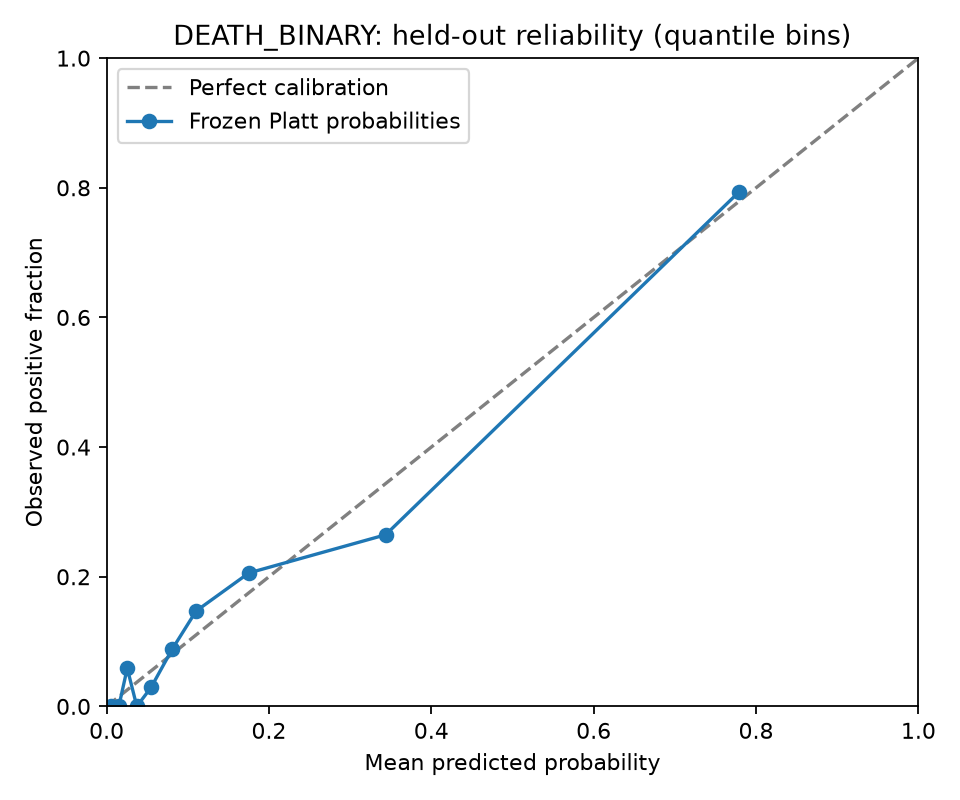
\includegraphics[width=\linewidth]{death_binary_reliability.png}\caption{Death}\end{subfigure}
\begin{subfigure}{.32\linewidth}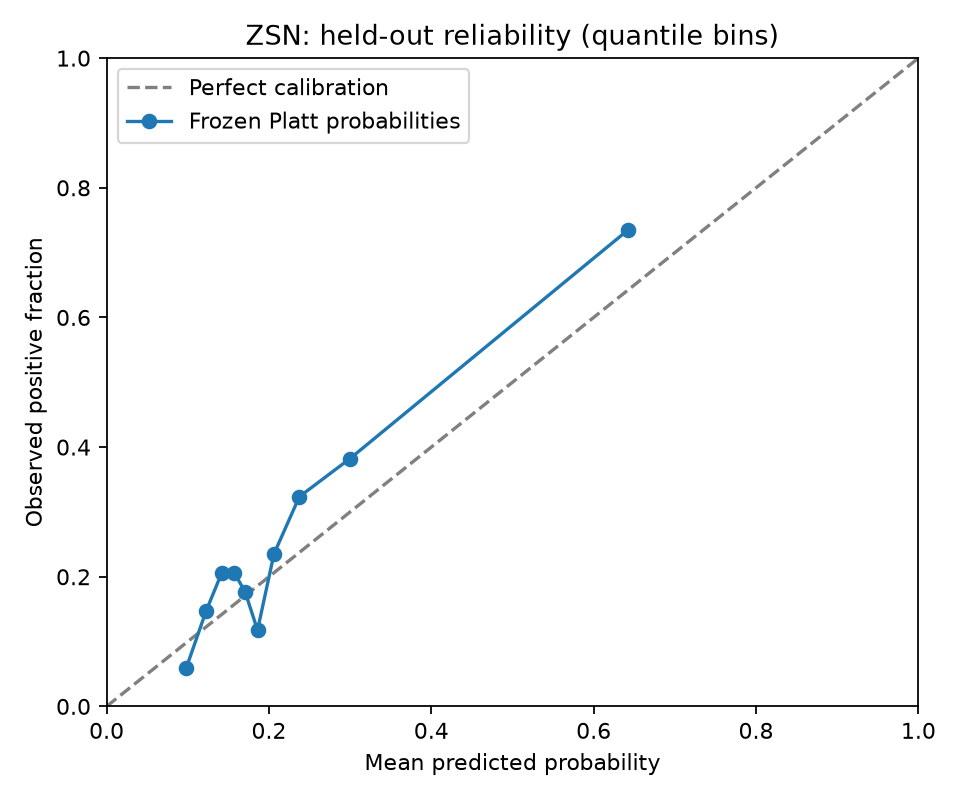
\includegraphics[width=\linewidth]{zsn_reliability.png}\caption{ZSN}\end{subfigure}
\begin{subfigure}{.32\linewidth}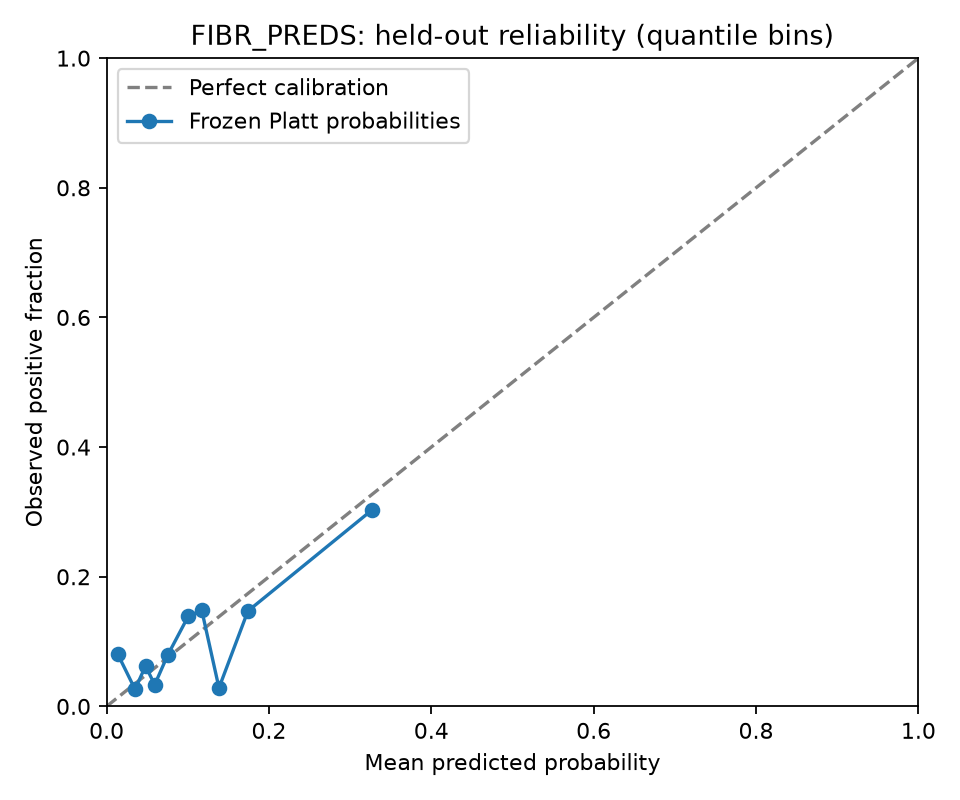
\includegraphics[width=\linewidth]{fibr_preds_reliability.png}\caption{FIBR\_PREDS}\end{subfigure}
\caption{Final test reliability diagrams for the frozen Platt predictions. These are descriptive test-set diagnostics and did not alter predictions. Source: T07 outputs.}\label{fig:testcal}
\end{figure}

The T07 report also provides decision curves from threshold probabilities 0.05--0.40 against treat-all and treat-none strategies. They are descriptive and do not select the frozen operating thresholds. Aggregate numeric results and run provenance are in \texttt{stage11\_t07\_outputs/}; the separate assignment probability export is \texttt{stage12\_t08\_outputs/submission.csv} with header \texttt{ID,LET\_IS,ZSN,FIBR\_PREDS}.
